\documentclass[a4paper,11pt,fleqn]{article}%fleqn pour aligner les equations à gauche
\usepackage{../../Styles/Cours}


\newcommand{\chnum}{Chapitre 02}
\newcommand{\chtitle}{Étude de la dynamique d'un système électrique}
\newcommand{\dtype}{Cours}
  
\begin{document}

\maketitle
\section{L'obtention des couleurs}
Les procédés de synthèse additive et soustractives reposent sur la structure de l'\oe il humain. Celui-ci perçoit les couleurs grâce à des récepteurs appelés cônes. Il en existe de trois types, chacun étant sensible à une longueur d'onde de la lumière particulière.
    \subsection{Synthèse additive}
    \begin{minipage}{0.68\textwidth}
        La superposition de trois \underline{lumières} colorées permet d'obtenir une infinité d'autres couleurs.\\
        À partir des trois couleurs primaires : le bleu, le rouge et le vert, il est donc possible de produire des couleurs secondaires par superposition : le cyan, le jaune et le magenta.\\
        La superposition des trois couleurs primaires donnant du blanc.
    \end{minipage}
    \begin{minipage}
        {0.3\textwidth}
        \begin{center}
            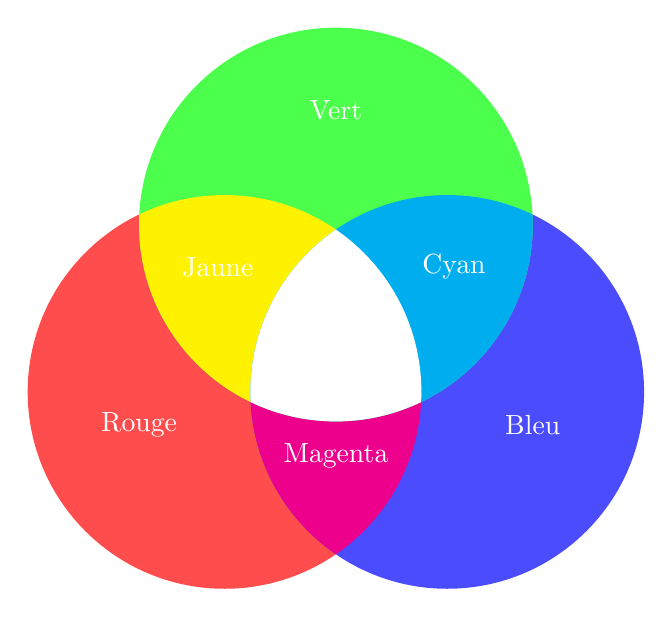
\begin{tikzpicture}[scale=1] 
\def\r{2.5};%rayon des cercles 
\newcommand{\R}{(0,0) ++(135:2) circle ({\r})}%rouge 
\newcommand{\B}{(0,0) ++(45:2) circle ({\r})}%bleu 
\newcommand{\G}{(0,0) ++(90:3.54) circle ({\r})}%vert 
\fill[color=red!70]\R;%disque rouge 
\fill[color=blue!70]\B;%disque bleu 
\fill[color=green!70]\G;%disque vert 
\begin{scope}%intersection bleu et rouge 
\clip \B; 
\fill[color=magenta] \R; 
\end{scope} 
\begin{scope}%intersection vert et rouge 
\clip \R; 
\fill[color=yellow] \G; 
\end{scope}
\begin{scope}%intersection bleu et vert 
\clip \B; 
\fill[color=cyan] \G; 
\end{scope}; 
\begin{scope}%blanc 
\clip \B; 
\clip \R; 
\fill[white] \G; 
\end{scope} 
\node[color=white] at (2.5,1){Bleu}; 
\node[color=white] at (-2.5,1){Rouge}; 
\node[color=white] at (0,5){Vert}; 
\node[color=white] at (1.5,3){Cyan}; 
\node[color=white] at (-1.5,3){Jaune}; 
\node[color=white] at (0,0.6){Magenta}; 
\end{tikzpicture}
        \end{center}
    \end{minipage}

    \subsection{Synthèse soustractive}
    \begin{minipage}{0.68\textwidth}
        La superposition de trois \underline{filtres} colorés permet d'obtenir une infinité d'autres couleurs.\\
        À partir des trois couleurs primaires : le cyan, le magenta et le jaune, il est donc possible de produire des couleurs secondaires par superposition : le bleu, le rouge et le vert.\\
        La superposition des trois couleurs primaires donnant du noir.
    \end{minipage}
    \begin{minipage}
        {0.3\textwidth}
        \begin{center}
            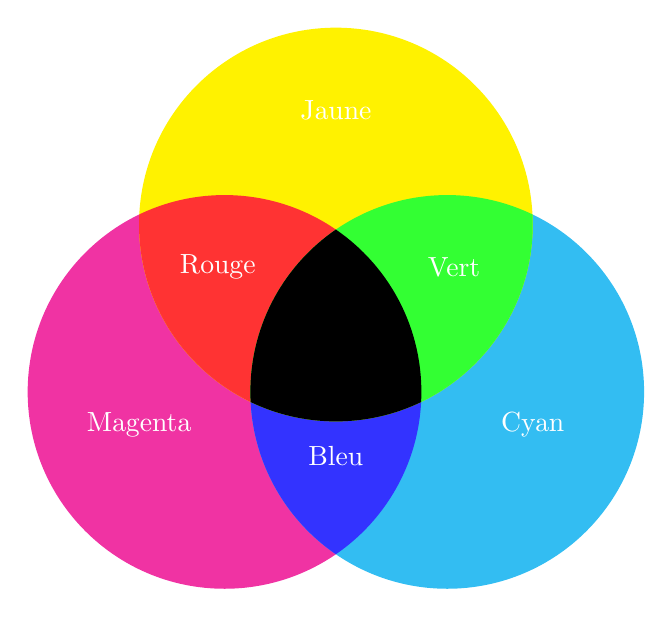
\begin{tikzpicture}[scale=1] 
\def\r{2.5};%rayon des cercles 
\newcommand{\M}{(0,0) ++(135:2) circle ({\r})}%magenta 
\newcommand{\CY}{(0,0) ++(45:2) circle ({\r})}%cyan 
\newcommand{\JA}{(0,0) ++(90:3.54) circle ({\r})}%jaune 
\fill[color=magenta!80]\M;%disque magenta 
\fill[color=cyan!80]\CY;%disque cyan 
\fill[color=yellow]\JA;%disque jaune 
\begin{scope}%intersection cyan et magenta 
\clip \M; 
\fill[color=blue!80] \CY; 
\end{scope} 
\begin{scope}%intersection magenta et jaune 
\clip \M; 
\fill[color=red!80] \JA; 
\end{scope} 
\begin{scope}%intersection jaune et cyan 
\clip \JA; 
\fill[color=green!80] \CY; 
\end{scope}; 
\begin{scope}%blanc 
\clip \M; 
\clip \JA; 
\fill[black] \CY; 
\end{scope} 
\node[color=white] at (2.5,1){Cyan}; 
\node[color=white] at (-2.5,1){Magenta}; 
\node[color=white] at (0,5){Jaune}; 
\node[color=white] at (1.5,3){Vert}; 
\node[color=white] at (-1.5,3){Rouge}; 
\node[color=white] at (0,0.6){Bleu}; 
%\node at (0,-1.5){Synthèse soustractive}; 
\end{tikzpicture}
        \end{center}
    \end{minipage}
\section{Couleur des objets}
    \subsection{Interaction entre lumière et objets}
    \begin{minipage}
        {0.68\textwidth}
        Selon la nature et les caractéristiques physiques des objets, l'interaction qu'ils auront avec la lumière incidente ne sera pas la même.\\
        Lorsqu'un objet reçoit une lumière incidente, il peut :
        \begin{itemize}
            \item absorber une partie de la lumière incidente ;
            \item réfléchir une partie de la lumière incidente ;
            \item transmettre une partie de la lumière incidente : elle traverse l'objet.
        \end{itemize}
        Dans la majorité des cas les trois phénomènes se produisent en même temps : en effet une partie de la lumière est absorbée par l'objet et une autre peut être transmise. Un objet coloré absorbe sa couleur complémentaire.
    \end{minipage}
    \begin{minipage}
        {0.3\textwidth}
        \begin{center}
            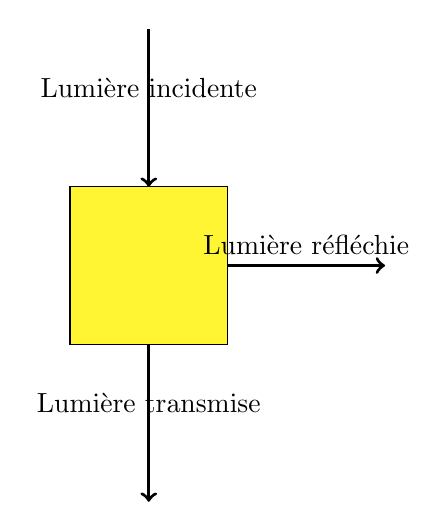
\begin{tikzpicture}[scale=1]
            %Lumiere incidente
            \filldraw[fill=yellow!80, draw=black] (-1,-1) -- (1,-1) -- (1,1) -- (-1,1) -- cycle;
            \draw[->,very thick] (0,3)--(0,1) node[midway,above] {Lumière incidente};
            \draw[->,very thick] (0,-1)--(0,-3) node[midway,above] {Lumière transmise};
            \draw[->,very thick] (1,0)--(3,0) node[midway,above] {Lumière réfléchie};
        \end{tikzpicture}
        \end{center}
    \end{minipage}
    \subsection{Perception des couleurs par l'être humain}
    L'\oe il d'un observateur va recevoir en provenance d'un objet, la lumière qu'il diffuse ou qu'il transmet. Dans l'\oe il, deux types de cellules permettent de discerner la couleur des objets :  les cônes qui détectent les couleurs et les bâtonnets qui sont sensibles à l'intensité lumineuse. Il existe trois types de cônes et chacun est spécialité pour une couleur primaire : bleu, rouge et vert.\\
    La couleur d'un objet va donc être interprété comme une combinaison des trois couleurs primaires par le cerveau.
    \subsection{Couleur réelle d'un objet}
    La couleur d'un objet dépend de deux paramètres : la couleur de la lumière incidente et la vision de l'observateur.
    \textit{Exemple :} Un objet cyan, quand il est éclairé par une lumière blanche, va apparaître noir lorsqu'il est éclairé en lumière rouge.\\
    On parle de la couleur réelle d'un objet lorsqu'il est éclairé par une lumière blanche et vu par un observateur dont l'\oe il est sensible aux trois couleurs primaires.
\end{document}
